\begin{itemize}
	\item {\textbf{Kratak opis:}  Istovara se roba i prebrojava ispravna istovarena roba. Vozach obaveshtava administratora o kolichini ispravne robe, nakon chega dobija fakturu rachuna. Ispostavlja rachun korisniku. Vozach dobija potpisan rachun. Shalje administratoru zavrshnu kopiju rachuna i upuc1uje se nazad.}
	\item{\textbf{Ucesnici:} Korisnik, Vozach , Administrator}
	\item{\textbf{Preduslovi:} Kamion je istovaren od strane korisnikove firme }
	\item{\textbf{Postuslovi}: Povratak vozacha}
	\item{\textbf{Osnovni tok:}  \begin{enumerate}
				\item {Vozach prebrojava kolichinu istovarene robe}
				\item{Vozach shalje administratoru potvrdu o kolichini istovarene robe}
				\item{Vozach dobija oformljen rachun}
				\item {Korisnik proverava i potpisuje}
				\item{Vozach shalje administratoru potvrdu o zavrshetku ispostavljanja rachuna}
	\end{enumerate}
			}
\item{\textbf{Alternativni tok:}
	 \begin{enumerate}
		\item[A{1}]{\textbf{Korisnik se ne nalazi na mestu istovara} 
			\begin{itemize}
				\item[A{1.1}]{Fiskalni rachun se ostavlja na istovarenom mestu, nakon chega c1e faktura biti prosled1ena logisticharu}
			\end{itemize}	
						}
	\end{enumerate}
		}
\item{\textbf{Podtokovi:} /}
\item{\textbf{Specijalni zahtevi:} 
			\begin{itemize}
				\item[S{1}]{Podrazumeva se da firme imaju usklad1en i dogovor nachin plac1anja}
				\item[S{2}]{Podrazumeva se da administrator ima shablon rachuna koji popunjava od informacija vozacha}
		\end{itemize}
	
}
\item{\textbf{Dodatne informacije:} 
					\begin{itemize}
						\item[D{1}]{Vozach nakon izvrshene naplate se oznachava kao da je zavrsio radno vreme, ne prati se njegov dalji povratak}
					\end{itemize}
}

\end{itemize}
\begin{figure}[h!]
	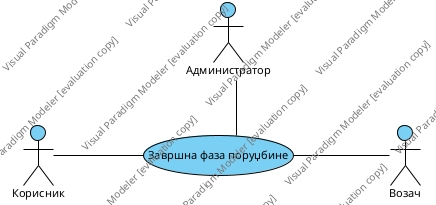
\includegraphics[scale=0.5]{Slike/UML/SUzavrsnaFazaPorudzbineUse Case Diagram.jpg}
	\centering
	\caption{Dijagram sluchaja upotrebe: Zavrshna faza porud2bine}
	\label{ucZavrsnaFaza}
\end{figure}

\newpage

\begin{figure}[h!]
	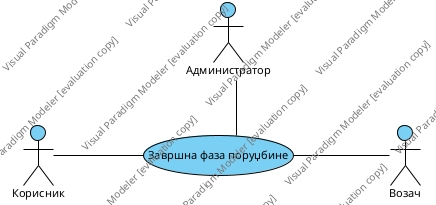
\includegraphics[scale=0.4]{Slike/UML/SUzavrsnaFazaPorudzbineUse Case Diagram.jpg}
	\centering
	\caption{Dijagram aktivnosti : Zavrshna faza narud2bine}
	\label{ucZavrsnaFazaAktivnost}
\end{figure}
\begin{figure}[h!]
	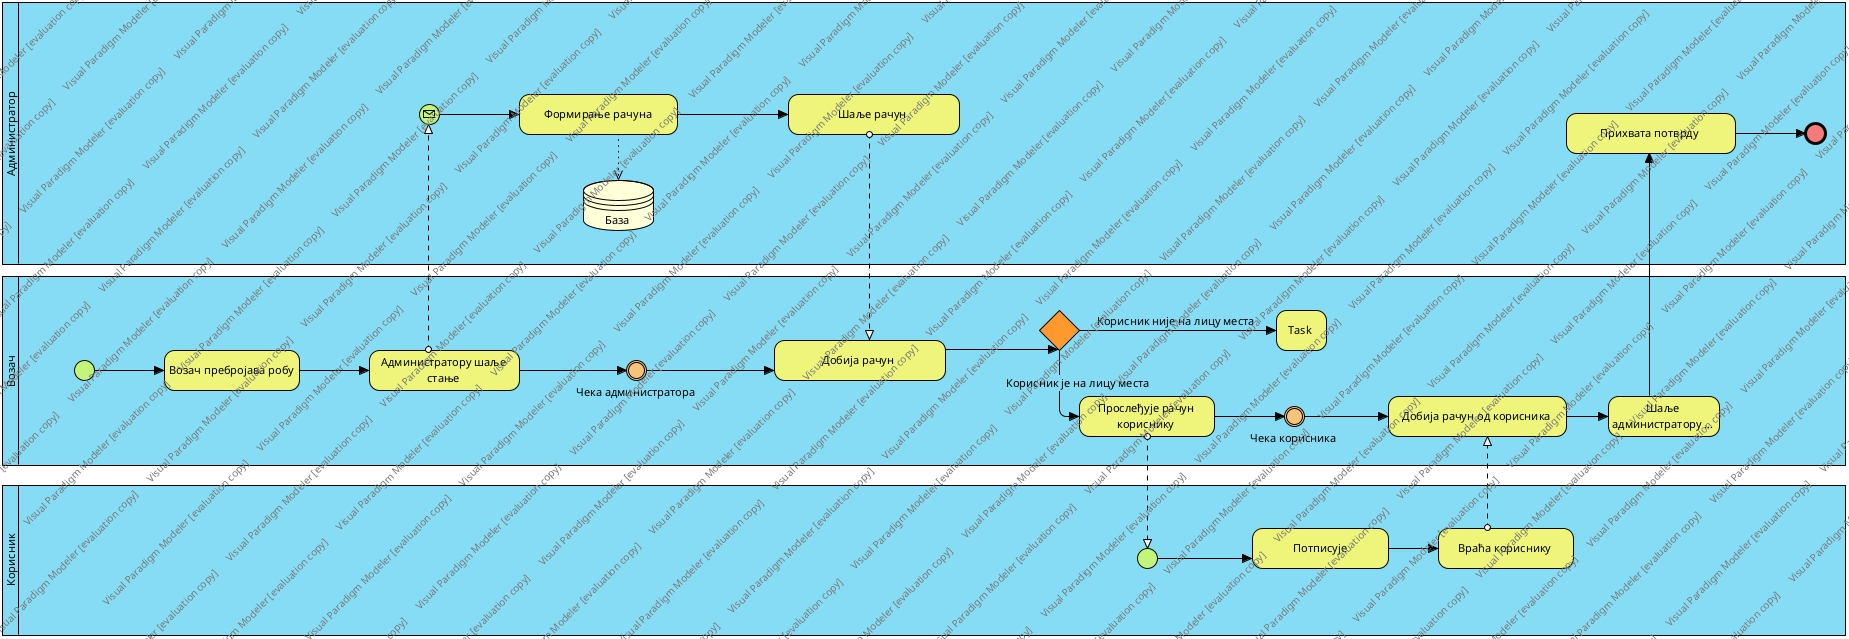
\includegraphics[scale=0.4]{Slike/BPMN/BPMNzavrsnaFazaPorudzbine.jpg}
	\centering
	\caption{Dijagram sekvenci : Zavrshna faza narud2bine}
	\label{ucZavrsnaFazaSekvence}
\end{figure}
\begin{figure}[h!]
	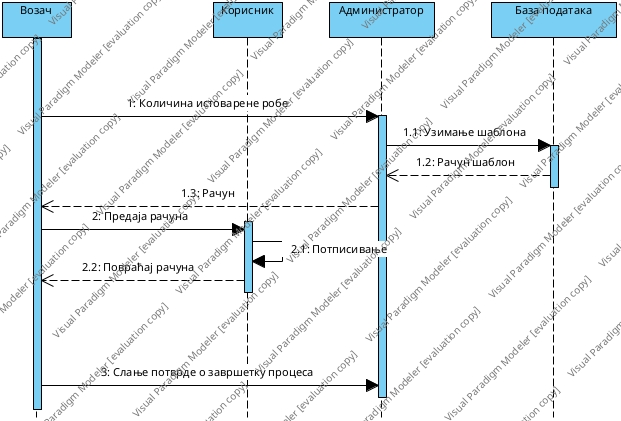
\includegraphics[scale=0.4]{Slike/DFD/SUzavrsnaFazaProudzbineSequence Diagram1.jpg}
	\centering
	\caption{Dijagram sekvenci : Zavrshna faza narud2bine}
	\label{ucZavrsnaFazaSekvence}
\end{figure}
